
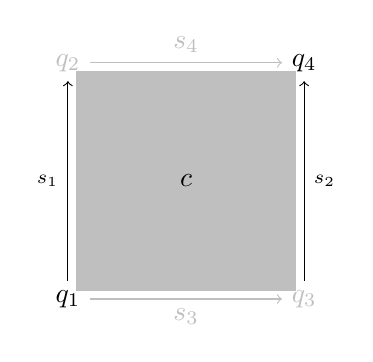
\begin{tikzpicture}[scale=1]
		
	\node (11) at (0,0) {$q_1$};
	\node (12) at (0,3) {$\textcolor{gray!50}{q_2}$};
	\node (21) at (3,0) {$\textcolor{gray!50}{q_3}$};
	\node (22) at (3,3) {$q_4$};
	
	\draw[draw = white, fill = gray!50] (0.1,0.1) rectangle (2.9,2.9);
	
	\node (c) at (1.5,1.5) {$c$};
	
	\path[->,font=\scriptsize]
		(11) edge node[left]{$s_1$} (12)
		(21) edge node[right]{$s_2$} (22);
		
	\path[->, gray!50]
		(11) edge node[below]{$s_3$} (21)
		(12) edge node[above]{$s_4$} (22);
			
\end{tikzpicture}

